\begin{figure}[hb!]
\centering
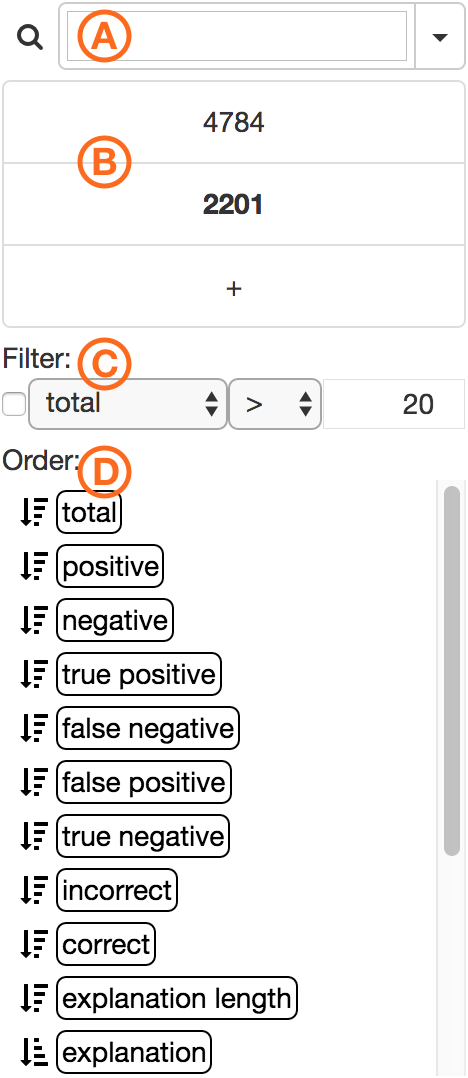
\includegraphics[width=0.45\linewidth]{fig/controls_annotated}
\caption{
The controls of the \tabB .
The first entry of the list of filtered data items (B) represents the full dataset and following entries show sizes after filter steps are applied.
The ``+" creates a new filter according to the current selection of explanations.
Explanations can be selected satisfying a condition (C) or by searching for features in the search box (A).
The sort order of explanations is defined by the list at the bottom (D).
}
\label{figs:controls}
\end{figure}